\documentclass{article}%[12pt, a4paper]{article}

\usepackage{ucs}
\usepackage[russian]{babel}
\usepackage{cmap}
\usepackage[utf8x]{inputenc}
\usepackage{amsthm}
\usepackage{amsmath}
\usepackage{amssymb}
\usepackage{graphicx}
\usepackage{float}
\usepackage{clrscode}
\usepackage{tocloft}
\usepackage[usenames]{color}
\usepackage[margin=20mm]{geometry}
\usepackage{sidecap}
\usepackage{url}
\usepackage{hyperref}

\frenchspacing



\begin{document}

\thispagestyle{empty}

\begin{frame}
  \maketitle
  \begin{center}
  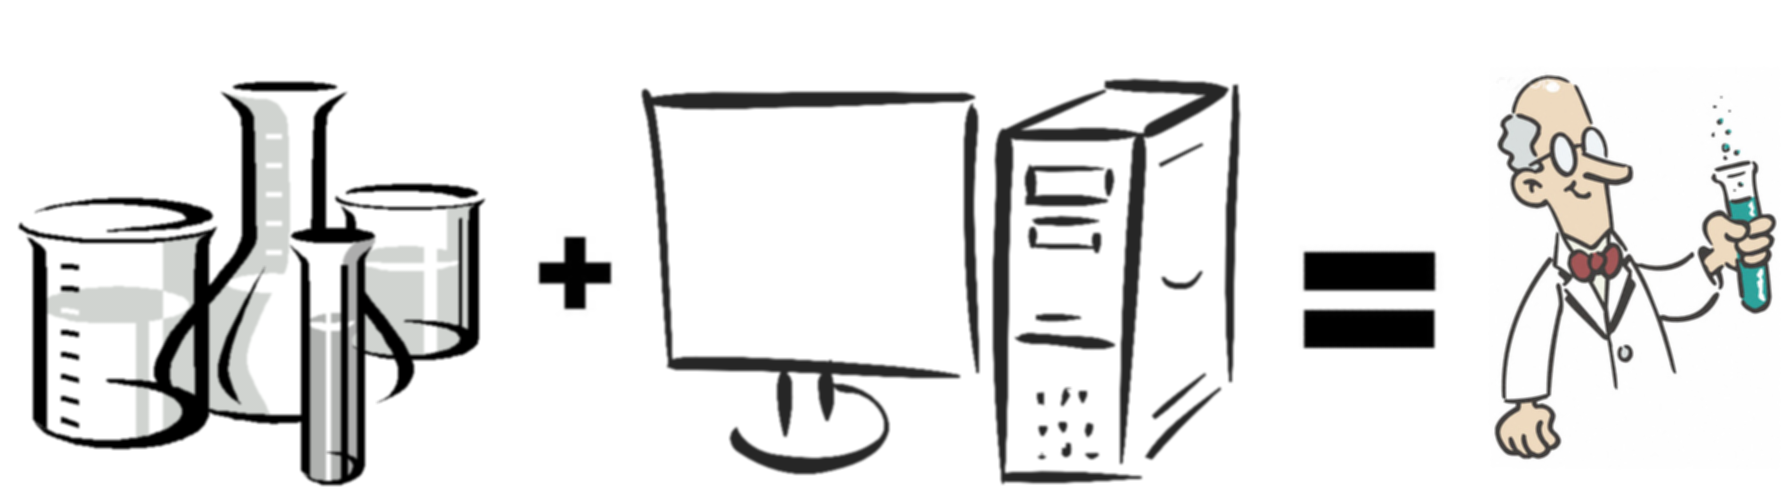
\includegraphics[scale=0.5]{images/title.png}
\end{center}
\end{frame}

\setcounter{page}{1}

\begin{frame}
  \frametitle{Содержание} 
  \tableofcontents
\end{frame}

\section{Введение}
\subsection{Определение}

\begin{frame}
  \frametitle{Введение}
  \framesubtitle{Определение(1)}

  \begin{columns}
    \begin{column}{0.5\textwidth}
       \begin{itemize}
         \item Химическая информатика
         \item Хемоинформатика
       \end{itemize}
    \end{column}
    \begin{column}{0.5\textwidth}
       \begin{itemize}
         \item Chemical informatics
         \item Chem-, chemo- informatics
       \end{itemize}
    \end{column}
  \end{columns}

  \begin{defn}[Ф.К.Браун, 1998]
     Хемоинформатика означает совместное использование информационных ресурсов для преобразования данных
     в информацию и информации в знания для быстрейшего принятия наилучших решений при поиске соединений
     в разработке лекарств и их оптимизации 
  \end{defn}

\end{frame}

\begin{frame}
  \frametitle{Введение}
  \framesubtitle{Определение(2)}

  \begin{defn}[Г.Пэриз, <<Новартис>>]
    Хемоинформатика это научная дисциплина, охватывающая дизайн, создание, организацию, управление, поиск, 
    анализ, распространение, визуализацию и использование химической информации
  \end{defn}

  \begin{defn}[И.Гастайгер]
    Хемоинформатика это применение методов информатики для решения химических проблем
  \end{defn}

  \begin{defn}[Р.Грин]
    Хемоинформатика - новое название старых проблем
  \end{defn}
 
\end{frame}

\subsection{Хемоинформатика и другие науки}

\begin{frame}
  \frametitle{Введение}
  \framesubtitle{Хемоинформатика и другие науки(1)}
  \begin{columns}
    \begin{column}{0.5\textwidth}
      \begin{itemize}
   \item  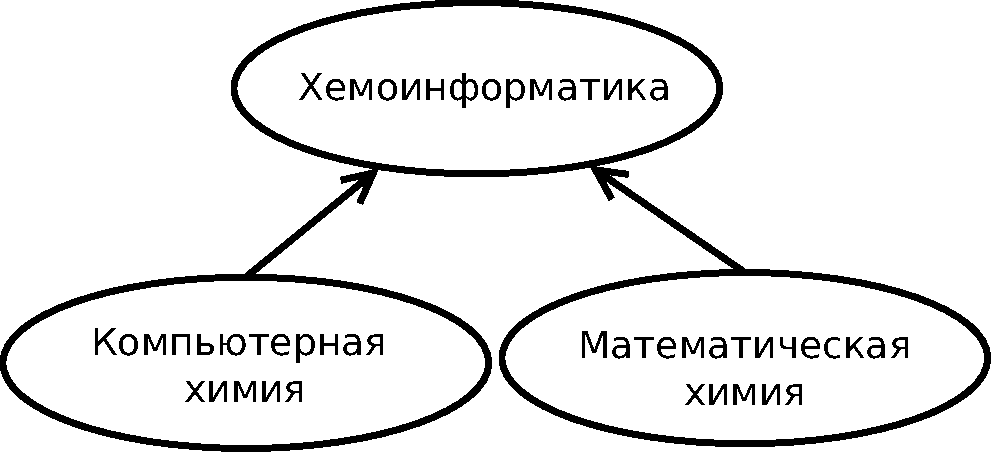
\includegraphics[scale=0.32]{images/Diagram1.pdf}
   \item  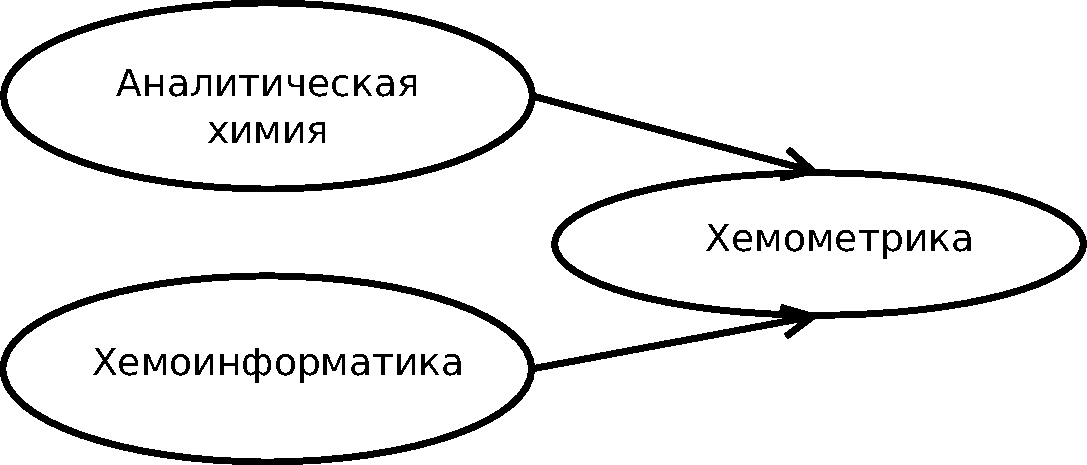
\includegraphics[scale=0.3]{images/Diagram3.pdf}
      \end{itemize}
    \end{column}
    \begin{column}{0.5\textwidth}      
      \begin{itemize}
      \item 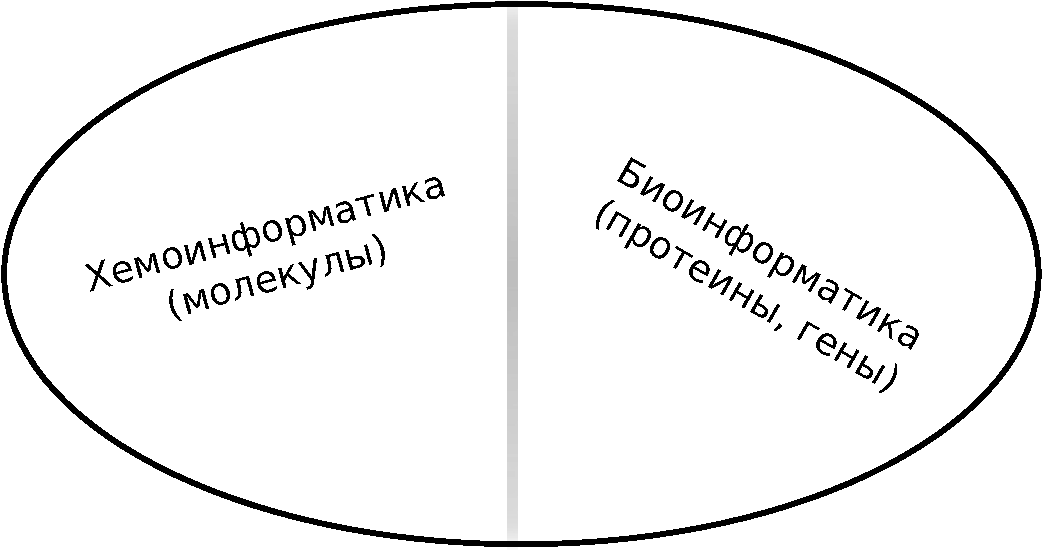
\includegraphics[scale=0.3]{images/Diagram2.pdf}
      \item 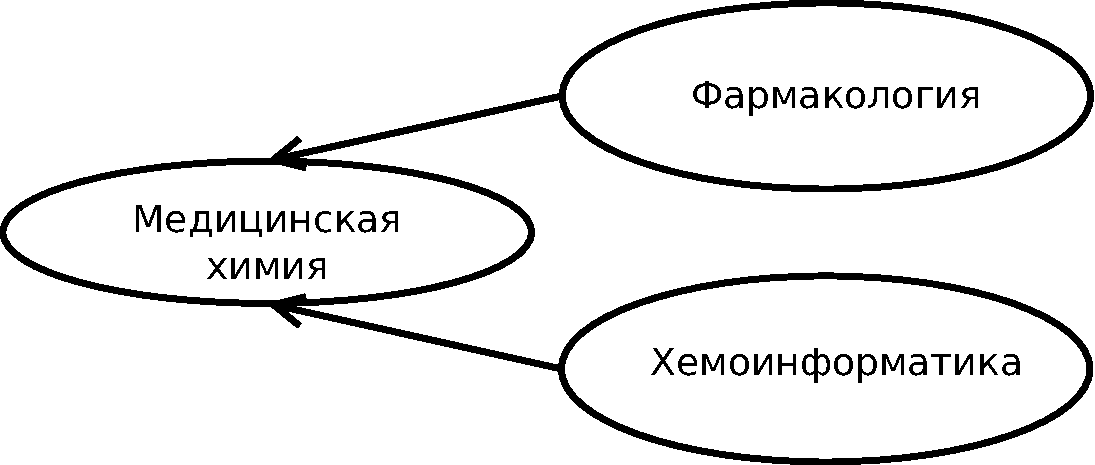
\includegraphics[scale=0.29]{images/Diagram4.pdf}
      \end{itemize}
    \end{column}
  \end{columns}
\end{frame}

\begin{frame}
  \frametitle{Введение}
  \framesubtitle{Хемоинформатика и другие науки(2)}

  \begin{center}
    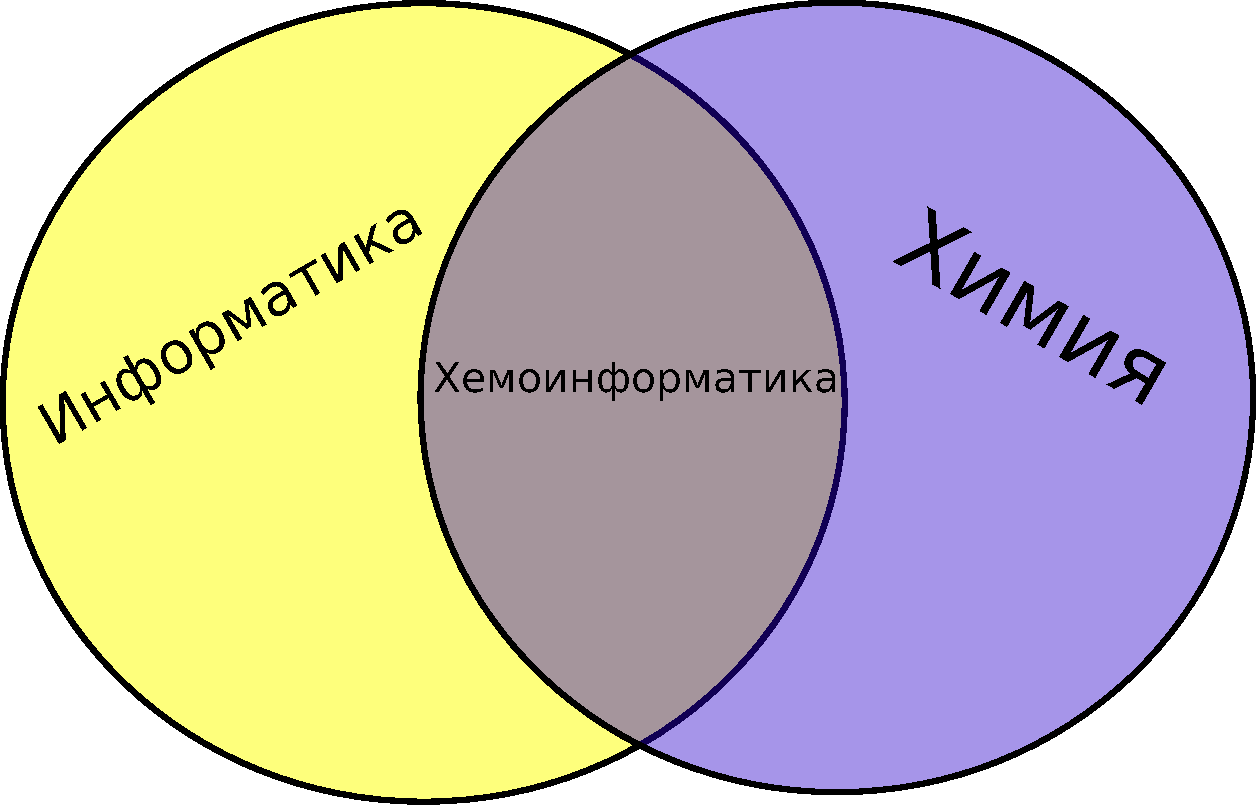
\includegraphics[scale=0.3]{images/Diagram5.pdf}
  \end{center}

  Основные используемые области информатики и математики:
  \begin{columns}
    \begin{column}{0.5\textwidth}
  \begin{itemize}
    \item Базы данных
    \item Интеллектуальный анализ данных
    \item Математическая статистика
   \end{itemize}
\end{column}
\begin{column}{0.5\textwidth}
  \begin{itemize}
   \item Машинное обучение
    \item Теория графов
    \item Компьютерная графика
      \end{itemize}

\end{column}
\end{columns}
\end{frame}

\section{Фундаментальные вопросы}
\begin{frame}
   \frametitle{Фундаментальные вопросы}
   \begin{columns}
      \begin{column}{0.5\textwidth}
      \begin{enumerate}
         \item Какое {\color{red}химическое соединение} обладает интересующим свойством? \\
            \emph{Свойство} $ \overset{QSPR\footnotemark}{\rightarrow} $ \emph{Структура}
         \item Как получить такое {\color{red}химическое соединение}? \\
            \emph{Исходные вещества} $ \rightarrow $ \emph{Соединение}
         \item Какое {\color{red}химическое соединение} получится в результате реакции? \\
            \emph{Реакция} $ \rightarrow $ \emph{Продукт}
      \end{enumerate}
      \end{column}
      \begin{column}{0.5\textwidth}
         
\includegraphics[scale=0.65]{images/question-marks2.png}
      \end{column}
   \end{columns}

\footnotetext{Quantative Structure-Property Relationship}

\end{frame}

\begin{frame}
  \frametitle{Причины появления хемоинформатики}
  \begin{columns}
    \begin{column}{0.5\textwidth}
  \begin{itemize}
    \item Огромное количество информации: миллионы соединений, миллионы публикаций
    \item Сложные химико-биологические связи
  \end{itemize}
   \end{column}
   \begin{column}{0.5\textwidth}
     \centering 
\includegraphics[scale=0.2]{images/sad.png} \\ 
     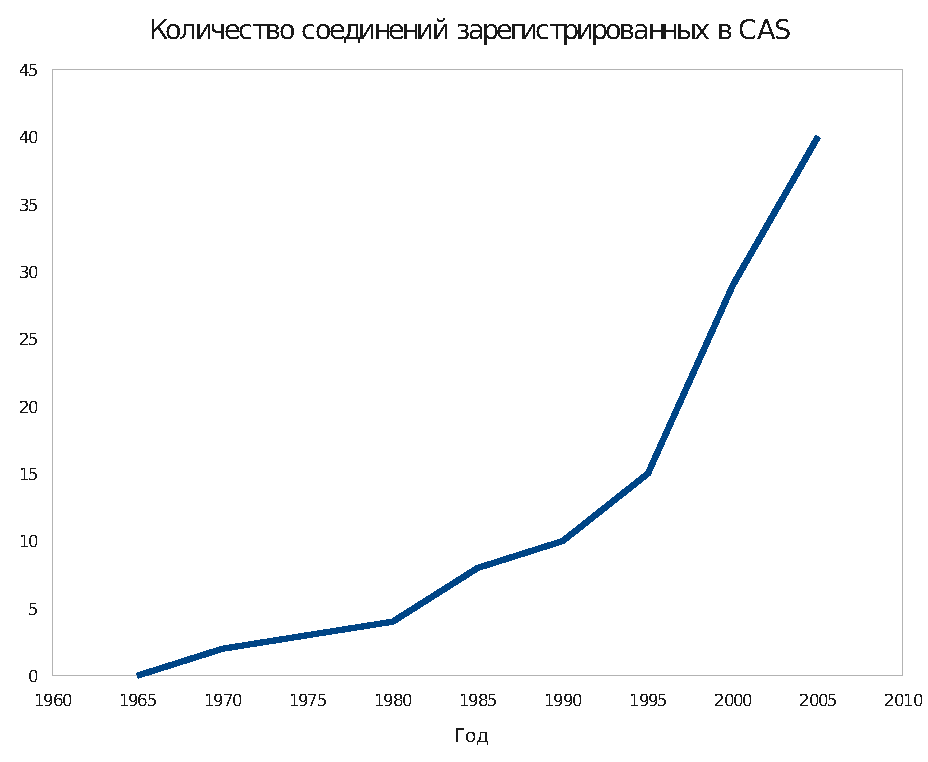
\includegraphics[scale=0.35]{images/graph.pdf}
   \end{column}
 \end{columns}

 \footnotetext{CAS: Chemical Abstracts Service, химическая реферативная служба}

\end{frame}

\section{Представление химической информации}
\subsection{Внутреннее}
\begin{frame}
  \frametitle{Представление химической информации}
  \framesubtitle{Внутреннее: модель молекулярного графа(1)}
   \begin{columns}
    \begin{column}{0.6\textwidth}
      \begin{tabular}{|c|c|}
      \hline Химия & Теория графов \\ \hline
      {\color{magenta}Молекула} & {\color{orange}Связный компонент} \\ \hline
      {\color{magenta}Атом} & {\color{orange}Вершина} \\ \hline
      {\color{magenta}Связь} & {\color{orange}Ребро} \\ \hline
      {\color{magenta}Название атома} & {\color{orange}Метка вершины} \\ \hline
      {\color{magenta}Порядок связи} & {\color{orange}Метка ребра} \\ \hline
      {\color{magenta}Валентность атома} & {\color{orange}Степень вершины} \\ \hline
      \end{tabular} \\
    \end{column}
    \begin{column}{0.2\textwidth}    
      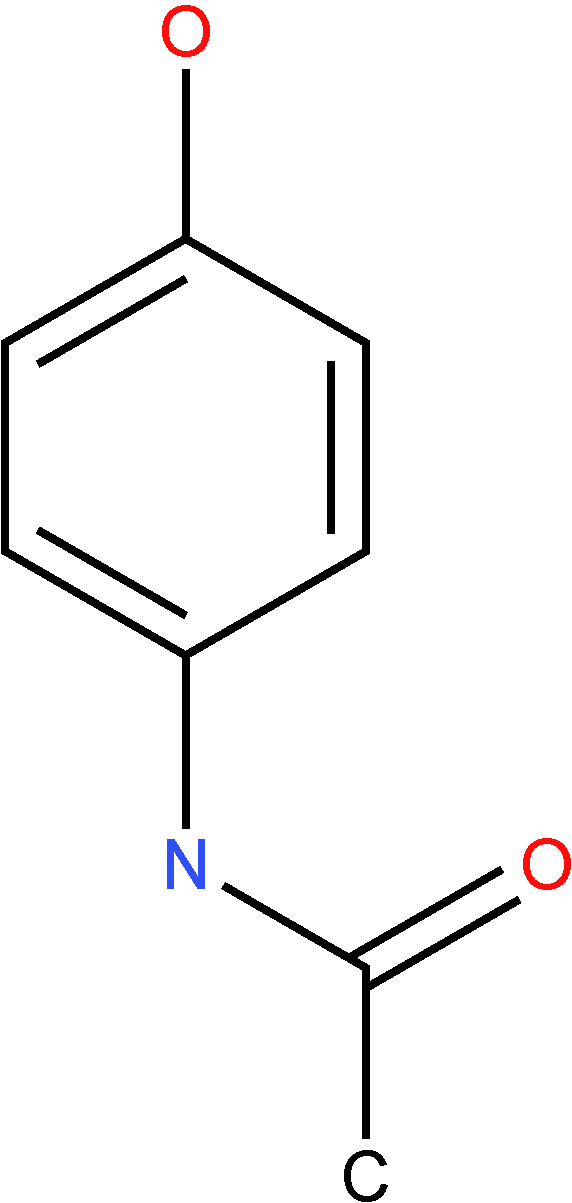
\includegraphics[scale=0.3]{images/Diagram6.pdf}      
    \end{column}
   \end{columns}
   Изоморфизм структурной формулы молекулы и молекулярного графа
\end{frame}

\begin{frame}
  \frametitle{Представление химической информации}
  \framesubtitle{Внутреннее: модель молекулярного графа(2)}
  \begin{center}
  \begin{tabular}{|m{5cm}|m{5cm}|}
      \hline Химия & Теория графов \\ \hline
      {\color{magenta}Свойство молекулы,} & {\color{orange}Инвариант графа} \\ 
      {\color{magenta}дескриптор молекулы} & \\ \hline
      {\color{magenta}Одинаковые молекулы} & {\color{orange}Изоморфные графы} \\ \hline
      {\color{magenta}Наличие определенного} & {\color{orange}Изоморфизм графа подграфу}  \\
      {\color{magenta}фрагмента в молекуле} & \\ \hline
      {\color{magenta}Поиск подструктуры} & {\color{orange}Поиск изоморфного} \\ & {\color{orange}подграфа} \\ \hline
      {\color{magenta}Пересечение молекул} & {\color{orange}Максимальный общий} \\ & {\color{orange}подграф} \\ \hline
      {\color{magenta}Порядок связи} & {\color{orange}Метка ребра} \\ \hline
      {\color{magenta}Топологическая группа} & {\color{orange}Группа автоморфизмов} \\ 
      {\color{magenta}симметрий} & {\color{orange}графа} \\ \hline
  \end{tabular} 
\end{center}
\end{frame}

\subsection{Внешнее}
\begin{frame}
  \frametitle{Представление химической информации}
  \framesubtitle{Внешнее: химические форматы файлов(1)}
  \begin{itemize}
    \item Строковое представление, \begin{tt}SMILES\end{tt}\footnotemark 
      \footnotetext{Simplified Molecular Input Line Entry Specification} 
      \begin{itemize}
        \item Метан $ CH_4 \overset{SMILES}{\rightarrow} C $
        \item Этанол $ C_2H_6O \overset{SMILES}{\rightarrow} CCO $
        \item Бензол $ C_6H_6 \overset{SMILES}{\rightarrow} C1=CC=CC=C1 $
      \end{itemize}
    \item Строковое представление, \begin{tt}InChi\end{tt}\footnotemark
        \footnotetext{IUPAC International Chemical Identifier}
        \begin{itemize}
          \item Этанол $ C_2H_6O \overset{InChi}{\rightarrow} InChi=1/C2H6O/c1-2-3/h3H,2H2,1H3 $
        \end{itemize}
      \item Представление с помощью языка разметки, \begin{tt}CML\end{tt}\footnotemark
          \footnotetext{Chemical Markup Language}
  \end{itemize}
\end{frame}

\begin{frame}
  \frametitle{Представление химической информации}
  \framesubtitle{Внешнее: химические форматы файлов(2)}
  \begin{itemize}
    \item Формат \begin{tt}XYZ\end{tt} $=$ метки атомов $+$ их координаты. Отражает геометрию молекулы.
    \item Табличное представление, \begin{tt}MDL\footnotemark Molfile\end{tt} \footnotetext{Molecular Design Limited, Inc.}
    \item Табличное представление, \begin{tt}SDF\end{tt}\footnotemark \footnotetext{Structure-Data File}
  \end{itemize}
  \begin{center}
   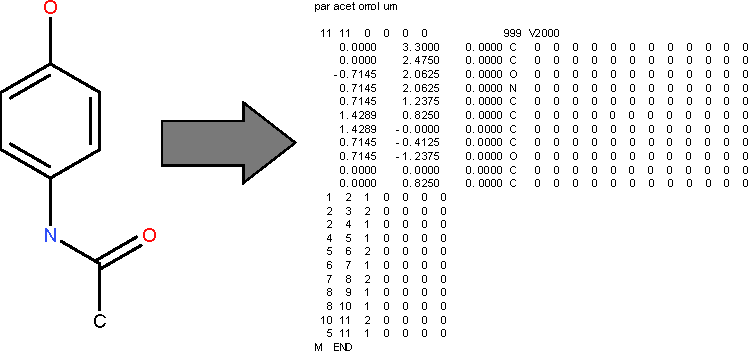
\includegraphics[scale=0.70]{images/parac.pdf}
  \end{center}
\end{frame}

\section{Навигация}

\begin{frame}
  
\end{frame}

\section{Известное программное обеспечение}
\begin{frame}
  \frametitle{Известное программное обеспечение}
\end{frame}

\section{Актуальные проблемы}
\begin{frame}
  \frametitle{Актуальные проблемы}
\end{frame}

\section{Заключение}
\begin{frame}
  \frametitle{Заключение}
\end{frame}

\section{Использованные ресурсы}

\begin{frame}
  \frametitle{Использованные ресурсы}
  \framesubtitle{Книги}
  \begin{enumerate}
    \item J.Gasteiger, T.Angel (2003). \emph{Chemoinformatics: A Textbook}     
    \item F.K.Brown (1998). \emph{Chemoinformatics: What is it and How does it Impact Drug Discovery}
    \item B.A.Bunin, B.Siesel, G.A.Morales, J.Bajorath (2007). \emph{Chemoinformatics: Theory, Practice, \& Products}
    \item A.R.Leach, V.J.Gillet (2007). \emph{An introduction to chemoinformatics}
  \end{enumerate}
\end{frame}

\begin{frame}
  \frametitle{Использованные ресурсы}
  \framesubtitle{Журналы, презентации, интернет}
  \begin{enumerate}
    \item Дмитрий Павлов, \emph{Навигация в мире органических соединений}, Компьютерные инструменты в образовании, 2010, №3 
    \item Сергей Кокорин, \emph{Заметки о Cheminfo'S. Strasbourg Summer School on Chemoinformatics.} 
    \item Материалы AACIMP-2008, курс ``Хемоинформатика'' \\ 
	       \url{http://summerschool.ssa.org.ua/}
    \item Noel O'Boyle, \emph{http://baoilleach.blogspot.com/}
    \item Википедия (русская, английская)
   \end{enumerate}

\end{frame}

\begin{frame}
   \begin{center}
   \LARGEСпасибо за внимание!
   \end{center}
\end{frame}

\end{document}


